% Options for packages loaded elsewhere
\PassOptionsToPackage{unicode}{hyperref}
\PassOptionsToPackage{hyphens}{url}
%
\documentclass[
]{article}
\usepackage{amsmath,amssymb}
\usepackage{iftex}
\ifPDFTeX
  \usepackage[T1]{fontenc}
  \usepackage[utf8]{inputenc}
  \usepackage{textcomp} % provide euro and other symbols
  \usepackage{lmodern}
  
\else % if luatex or xetex
  \usepackage{unicode-math} % this also loads fontspec
  \defaultfontfeatures{Scale=MatchLowercase}
  \defaultfontfeatures[\rmfamily]{Ligatures=TeX,Scale=1}
\fi
\usepackage{lmodern}
\ifPDFTeX\else
  % xetex/luatex font selection
\fi
% Use upquote if available, for straight quotes in verbatim environments
\IfFileExists{upquote.sty}{\usepackage{upquote}}{}
\IfFileExists{microtype.sty}{% use microtype if available
  \usepackage[]{microtype}
  \UseMicrotypeSet[protrusion]{basicmath} % disable protrusion for tt fonts
}{}
\makeatletter
\@ifundefined{KOMAClassName}{% if non-KOMA class
  \IfFileExists{parskip.sty}{%
    \usepackage{parskip}
  }{% else
    \setlength{\parindent}{0pt}
    \setlength{\parskip}{6pt plus 2pt minus 1pt}}
}{% if KOMA class
  \KOMAoptions{parskip=half}}
\makeatother
\usepackage{xcolor}
\usepackage[margin=1in]{geometry}
\usepackage{graphicx}
\makeatletter
\def\maxwidth{\ifdim\Gin@nat@width>\linewidth\linewidth\else\Gin@nat@width\fi}
\def\maxheight{\ifdim\Gin@nat@height>\textheight\textheight\else\Gin@nat@height\fi}
\makeatother
% Scale images if necessary, so that they will not overflow the page
% margins by default, and it is still possible to overwrite the defaults
% using explicit options in \includegraphics[width, height, ...]{}
\setkeys{Gin}{width=\maxwidth,height=\maxheight,keepaspectratio}
% Set default figure placement to htbp
\makeatletter
\def\fps@figure{htbp}
\makeatother
\setlength{\emergencystretch}{3em} % prevent overfull lines
\providecommand{\tightlist}{%
  \setlength{\itemsep}{0pt}\setlength{\parskip}{0pt}}
\setcounter{secnumdepth}{5}
\usepackage{caption}
\usepackage{subcaption}
\usepackage{multirow}
\usepackage{float}
\restylefloat{table}
\let\oldtable\table
\let\endoldtable\endtable
\renewenvironment{table}[1][H]{\oldtable[H]}{\endoldtable}
\usepackage{fancyhdr}
\pagestyle{fancy}
\fancyhf{}
\fancyhead[L]{\textbf{2025-05-24}}
\fancyhead[C]{\textbf{Term Project in Econometrics of Time Series}}
\fancyhead[R]{\textbf{Gereon Staratschek}}
\fancyfoot[C]{\thepage}
\usepackage{booktabs}
\usepackage{longtable}
\usepackage{array}
\usepackage{multirow}
\usepackage{wrapfig}
\usepackage{float}
\usepackage{colortbl}
\usepackage{pdflscape}
\usepackage{tabu}
\usepackage{threeparttable}
\usepackage{threeparttablex}
\usepackage[normalem]{ulem}
\usepackage{makecell}
\usepackage{xcolor}

\ifLuaTeX
  \usepackage{selnolig}  % disable illegal ligatures
\fi
\usepackage{bookmark}
\IfFileExists{xurl.sty}{\usepackage{xurl}}{} % add URL line breaks if available
\urlstyle{same}
\hypersetup{
  pdftitle={Macroeconometrics - UK variables report},
  pdfauthor={Souleymane Faye \& Gereon Staratschek},
  hidelinks,
  pdfcreator={LaTeX via pandoc}}
  
  \captionsetup{font=large}
  
  \usepackage{booktabs}
\usepackage{siunitx}
\usepackage{multirow}
  
\title{Term Project in Introduction to Econometrics of Time Series \\[1.5ex] 
{\Large An analysis of the United Kingdom GDP, Trade Balance, and Exchange Rate, 1955-2024}}
\author{Souleymane \textsc{Faye} \& Gereon \textsc{Staratschek}}
\date{2025-05-24}

\begin{document}
\maketitle

\section{Introduction}

In this project, we aim to analyze the development of the Gross Domestic
Product (GDP), exchange rates, and trade balance of the United Kingdom
(UK). We collect our data from the OECD open data portal. We use data on
a quarterly basis, starting latest in 1997. This period covers important
financial events such as the Global Financial Crisis (GFC) in 2007, the
Brexit referendum in 2016 and UK's final EU leave in 2020 as well as the
COVID-19 pandemic from 2020-2022.

\section{Univariate Analysis}

\subsection{Macro trends}

Figure 1 illustrates the evolution of the UK’s macroeconomic indicators—GDP, Trade Balance, 
and Exchange Rate—in both levels and first differences.

\paragraph*{Trend Dynamics and Structural Breaks in Level Series.} 
Data on UK's GDP, available on a quarterly basis
since 1955, exhibits a clear, upwards trajectory with only a few
shocks such as the 2007 financial crisis or the 2020 COVID-19 pandemic 
interrupting the general trend. Hence, the GDP of the UK is clearly not
stationary. However, the trend seems to be linear, suggesting that the
first-differences time series of the GDP might be stationary. Similarly, data on 
the trade balance is available on a quarterly basis starting in 1955.We see that 
the trade balance fluctuates around 0 until the 1990s where a negative trend seems to set
in continueing until the 2010s, when trade balance starts fluctuating
around a low, negative value. However, since the observed spikes are
getting much bigger over time, we also see an increase in fluctuation
around the respective stationary mean.

\begin{figure}[H]

\caption{\large \textsc{Trends in GDP, Trade Balance, and Exchange Rate}}\label{fig:trends-plot}

{\centering \includegraphics[width=0.8\linewidth]{../figures/uk_macro_levels_and_differences.png} 

}

{\footnotesize {\textit{Notes}: This figure presents levels (top row) and 
first differences (bottom row) of key UK macroeconomic indicators: real GDP 
(left), trade balance (center), and exchange rate against the US dollar (right),
from 1955 to 2023. All series are shown alongside Hodrick-Prescott (HP) trends 
with a smoothing parameter of $\lambda=1600$.  \\ \textit{Source}: Authors' 
computation from the UK Statistical Office.
} }

\end{figure}
Hence, the data seems to be
stationary in the beginning and in the end with a negative trend being
observed between the 1990s and the 2010s. Data on the exchange rate is available since
1997 on a quarterly basis. It exhibits stationarity between 1997 and
2007, as well as from 2007 onwards. In 2007, a shock seems to have
shifted the mean of the stationary process downwards. The bottom row highlights first-differenced series, which strip away trends to 
reveal stationary fluctuations and cyclical patterns, supporting the idea that 
differencing mitigates non-stationarity. Across all panels, Hodrick-Prescott 
filtered trends ($\lambda=1600$, standard for quarterly data) visually disentangle 
long-term trajectories from cyclical noise.

\subsection{Unit roots and stationarity tests}

In this section, we aim to formally conduct stationarity tests for the
series. As explained in the last section, we have reason to doubt that
our series are entirely stationary. However, for our analysis, we are
relying on stationarity properties of the series. Hence, after
identifying the non-stationary series formally, we will conduct the
first-difference transformation to obtain stationary series for our
analysis.

Table 1 presents the results of unit root and stationarity tests for our variables of interest, 
analyzed in both levels and first differences. The Augmented 
Dickey-Fuller (ADF), Phillips-Perron (PP), and Elliott, Rothenberg and Stock (ERS DF-GLS) tests evaluate the 
null hypothesis of a unit root (non-stationarity), while the Kwiatkowski-Phillips-Schmidt-Shin (KPSS) test assesses 
the null of stationarity. For GDP, the level series exhibits non-stationarity 
across all tests (e.g., ADF p-value = 0.353, KPSS statistic = 4.732*), but its 
first-differenced series shows strong evidence of stationarity (ADF statistic =
-8.020*, KPSS = 0.086). Similarly, the trade balance in levels displays 
persistent non-stationarity (KPSS = 3.395*), with stationarity achieved after 
first differencing (ADF = -8.171*). The exchange rate shows mixed results in 
levels (e.g., ADF p-value = 0.418), but clear stationarity in differences
(PP = -82.885***)

\begin{table}[!htbp]
\centering
\caption{\textsc{Unit Root and Stationnary Test Results}}
\label{tab:unit_root}
\begin{tabular}{@{} l cccc @{}}
\\[-1.8ex] \hline 
\hline  \\[-1.8ex] 
 & \multicolumn{4}{c}{Test Statistics} \\
\cmidrule(lr){2-5}
Series/Test & ADF & PP & ERS DF-GLS & KPSS \\
\midrule

\multicolumn{5}{@{}l}{Gross Domestic Product} \\
\cmidrule(lr){1-5}
Levels & $-2.531^{}$ $(0.353)$ & $-21.533^{***}$ $(0.048)$ & $3.074$ & $4.732^{***}$ \\
Differences & $-8.020^{***}$ $(0.010)$ & $-321.613^{***}$ $(0.010)$ & $-7.941^{***}$ & $0.086$ \\
\addlinespace

\multicolumn{5}{@{}l}{Trade Balance} \\
\cmidrule(lr){1-5}
Levels & $-2.225^{}$ $(0.481)$ & $-157.415^{***}$ $(0.010)$ & $-0.672$ & $3.395^{***}$ \\
Differences & $-8.171^{***}$ $(0.010)$ & $-300.088^{***}$ $(0.010)$ & $-12.912^{***}$ & $0.035$ \\
\addlinespace

\multicolumn{5}{@{}l}{Exchange Rate} \\
\cmidrule(lr){1-5}
Levels & $-2.382^{}$ $(0.418)$ & $-13.158$ $(0.354)$ & $-1.415$ & $1.754^{***}$ \\
Differences & $-5.041^{***}$ $(0.010)$ & $-82.885^{***}$ $(0.010)$ & $-2.188$ & $0.084$ \\
\hline \hline 
\end{tabular}

\vspace{0.2cm}
\begin{minipage}{\textwidth}
\scriptsize
\textit{Notes}: Null hypotheses—ADF/PP/ERS: series has a unit root 
(non-stationary); KPSS: series is stationary. To establish stationarity: reject
ADF/PP/ERS null (significant ***/**) \textit{and} fail to reject KPSS null 
(statistic $<$ critical value). P-values in parentheses. Critical values (1\% level): ADF/PP = $-3.43$, 
ERS DF-GLS = $-2.57$, KPSS = $0.739$. $^{***}p<0.01$, $^{**}p<0.05$. 
First differences calculated as $\Delta y_t = y_t - y_{t-1}$. 

\textit{Source}: Author's calculations using data from the UK Statistical Office.
\end{minipage}
\end{table}

We highlight that first-differencing effectively mitigates
non-stationarity, as evidenced by statistically significant rejections of
unit root hypotheses (***p<0.01) and failure to reject KPSS stationarity for 
differenced series.These results justify the use of differenced series for subsequent analysis, 
ensuring compliance with the stationarity assumptions underlying any further 
econometric treatment. Critical values and p-values are reported to validate the robustness
of conclusions.

\subsection{Model Estimation}

Next, we proceed to the model estimation.

\paragraph*{Statistical Models.}

Denote \( \nabla y_t = y_t - y_{t-1} \) the first-difference operator. We write
down three statistical models to guide our analysis. The univariate trade balance MA (4) model writes
\begin{equation}
        \nabla tb_t = \theta_1 \epsilon_{t-1} + \theta_2 \epsilon_{t-2} + \theta_3 \epsilon_{t-3} + \theta_4 \epsilon_{t-4} + \epsilon_t
    \end{equation}
     where \( tb_t \) denotes trade balance and $(\epsilon_t)_{1,..., T}$ is the innovation process.
    
The exchange rate AR (1) model is 
    \begin{equation}
        \nabla e_t = \phi_1 \nabla y_{t-1} + \nu_t
    \end{equation}
     where \( e_t \) represents exchange rate and $(\nu_t)_{1,..., T}$ is the innovation process 
The GDP univariate ARIMA (1,1,4) model with drift writes
    \begin{equation}
        \nabla y_t = c + \phi_1 \nabla y_{t-1} + \sum_{i=1}^4 \theta_i \gamma_{t-i} + \gamma_t
    \end{equation}
     where \( y_t \) is GDP and $(\gamma_t)_{1,..., T}$ is the innovation process.

\paragraph*{Estimation.} Table 2 shows the results of our estimations. We find that the Trade Balance 
has significant MA terms at the 1\% level (\( \theta_1 = -0.775^{***},\ \theta_4 = 0.278^{***} \)) 
indicate strong short- and long-lagged shock persistence. As for the exchange rate,
The autoregressive term (\( \phi_1 = 0.259^{***} \)) suggests moderate persistence 
in differenced exchange rate movements. GDP's key drivers include the AR(1)
term (\( \phi_1 = 0.489^{**} \)) and MA terms (\( \theta_1 = -0.770^{***},\ 
\theta_4 = -0.241^{***} \)), with a large intercept (\( c = 1832.987^{***} \)) 
reflecting persistent upward drift. The models
demonstrate heterogeneous dynamics: Trade balance exhibits complex error correction, 
exchange rate shows momentum effects, and GDP combines trend persistence with 
multi-period shock absorption. 

\begin{table}[htbp]
\centering
\caption{\textsc{ARIMA Model Estimates}}
\label{tab:arima}
\small
\begin{tabular}{@{} >{}l *{6}{S} @{}}
\\[-1.8ex] \hline \hline \\[-1.8ex] 
 & \multicolumn{2}{c}{Trade Balance} & \multicolumn{2}{c}{Exchange Rate} & \multicolumn{2}{c}{GDP} \\
\cmidrule(l{5pt}r{5pt}){2-3} \cmidrule(l{5pt}r{5pt}){4-5} \cmidrule(l{5pt}r{5pt}){6-7}
Component & {Coeff.} & {SE} & {Coeff.} & {SE} & {Coeff.} & {SE} \\
\midrule

AR(1)              & {--}          & {--}        & 0.259$^{***}$  & 0.092        & 0.489$^{**}$    & 0.202        \\
\addlinespace[0.5em]
MA(1)              & -0.775$^{***}$ & 0.057       & {--}           & {--}         & -0.770$^{***}$  & 0.199        \\
\addlinespace[0.5em]
MA(2)              & -0.100        & 0.074       & {--}           & {--}         & 0.093           & 0.093        \\
\addlinespace[0.5em]
MA(3)              & -0.030        & 0.080       & {--}           & {--}         & 0.135$^{*}$     & 0.075        \\
\addlinespace[0.5em]
MA(4)              & 0.278$^{***}$  & 0.064       & {--}           & {--}         & -0.241$^{***}$  & 0.061        \\
\addlinespace[0.5em]
Intercept          & {--}          & {--}        & {--}           & {--}         & 1832.987$^{***}$ & 232.754      \\

\hline \hline \\[-1.8ex] 
\end{tabular}

\vspace{0.4cm}
\begin{minipage}{\textwidth}
\footnotesize
\textit{Notes:} Coefficient estimates (Coeff.) with standard errors (SE). 
{--} = Component not included in model. Significance levels: $^{***}p<0.01$, $^{**}p<0.05$, $^{*}p<0.1$. 
AR = Autoregressive term, MA = Moving Average term. GDP intercept in original units. 
\textit{Source:} Author's calculations using UK Statistical Office data.
\end{minipage}
\end{table}

\subsection{Forecasting}

Table 3 reports forecast accuracy 
metrics for the first-differenced GDP, Trade Balance, and Exchange Rate series, 
calculated on the training set. The GDP series exhibits large absolute errors,
with a Root Mean Squared Error (RMSE) of 9,021.2 and a Mean Absolute Error (MAE)
of 3,505.4, while its Mean Absolute Scaled Error (MASE) of 0.77 suggests 
comparative performance relative to a benchmark. For the Trade Balance, the 
RMSE of 4,513.0 and MAE of 2,255.2 are accompanied by undefined percentage 
errors (MPE and MAPE), likely due to zero-crossings in the differenced series.
The Exchange Rate demonstrates smaller-scale errors, with an RMSE of 0.035 and 
MAE of 0.027, alongside percentage errors exceeding 100\%. Residual diagnostics
show near-zero first-order autocorrelation (ACF1) across all series, ranging 
from -0.003 for GDP to 0.006 for the Trade Balance. The MASE values, all below 
1, indicate that the models improve upon a naive forecast. These metrics reflect
the distinct scaling and volatility profiles of the macroeconomic series under study.

\begin{table}[htbp]
\centering
\caption{\textsc{Forecast Accuracy Metrics for First-Differenced Series}}
\label{tab:accuracy}
\footnotesize
\begin{tabular}{@{} l *{2}{S[table-format=-3.1]} S[table-format=4.1] S[table-format=-3.1] S[table-format=3.1] S[table-format=1.3] S[table-format=-1.3] @{}}
\\[-1.8ex]\hline \hline \\[-1.8ex] 
\textbf{Series} & \multicolumn{1}{c}{\textbf{ME}} & \multicolumn{1}{c}{\textbf{RMSE}} & \multicolumn{1}{c}{\textbf{MAE}} & \multicolumn{1}{c}{\textbf{MPE}} & \multicolumn{1}{c}{\textbf{MAPE}} & \multicolumn{1}{c}{\textbf{MASE}} & \multicolumn{1}{c}{\textbf{ACF1}} \\
\midrule
GDP & -30.6 & 9021.2 & 3505.4 & -106.5 & 452.6 & 0.770 & -0.003 \\[2.5ex] 
Trade Balance & -196.1 & 4513.0 & 2255.2 & {--} & {--} & 0.686 & 0.006 \\[2.5ex] 
Exchange Rate & -0.001 & 0.035 & 0.027 & 137.8 & 152.9 & 0.682 & -0.008 \\
\hline \hline \\[-1.8ex] 
\end{tabular}

\vspace{0.2cm}
\begin{minipage}{\textwidth}
\scriptsize
\textit{Notes:} All metrics calculated on training set. Scaling factors: 
GDP RMSE/MAE in original units ($x10^{-3}$), Exchange Rate ME ($x10^{-3}$). 
"{--}" indicates infinite values due to zero-base percentage calculations. 
ME: Mean Error, RMSE: Root Mean Squared Error, MAE: Mean Absolute Error, 
MPE: Mean Percentage Error, MAPE: Mean Absolute Percentage Error, 
MASE: Mean Absolute Scaled Error, ACF1: Lag-1 Autocorrelation.

\textit{Sources:} XX.
\end{minipage}
\end{table}

Figure \ref{fig:forecast_results} compares the true quarterly GDP change (black line) to the 
ARIMA model’s fitted values (dashed blue line). The model seems to fit the real 
data generally quite well. Important deviations occur when huge spikes occur in 
the true data such as the COVID-19 spike around 2020. Here, the model predictions 
severely underestimate the real development. Additionally, small deviations occur 
around turning points but overall, the blue and black lines are quite close to each 
other, indicating a good in-sample fit. Note that although the MPE and MAPE errors 
are quite high, these percentage metrics blow up as the GDP growth is close to 0. 
Hence, the relatively high values of these specific accuracy metrics do not alarm us.
Looking at the out-of-sample forecast, the model predicts GDP growth to continue 
hovering around a constant mean close to zero. However, we face rising uncertainty 
of our predictions as we go further into the future, showing the increasing 
variance of the Best Linear Forecast errors.

\begin{figure}[htbp]
    \centering
        \caption{\textsc{Forecast performance for UK GDP, Exchange Rate, and Trade Balance}}
    \label{fig:forecast_results}
    % GDP: In-sample and Forecast
    \begin{subfigure}[b]{0.45\textwidth}
        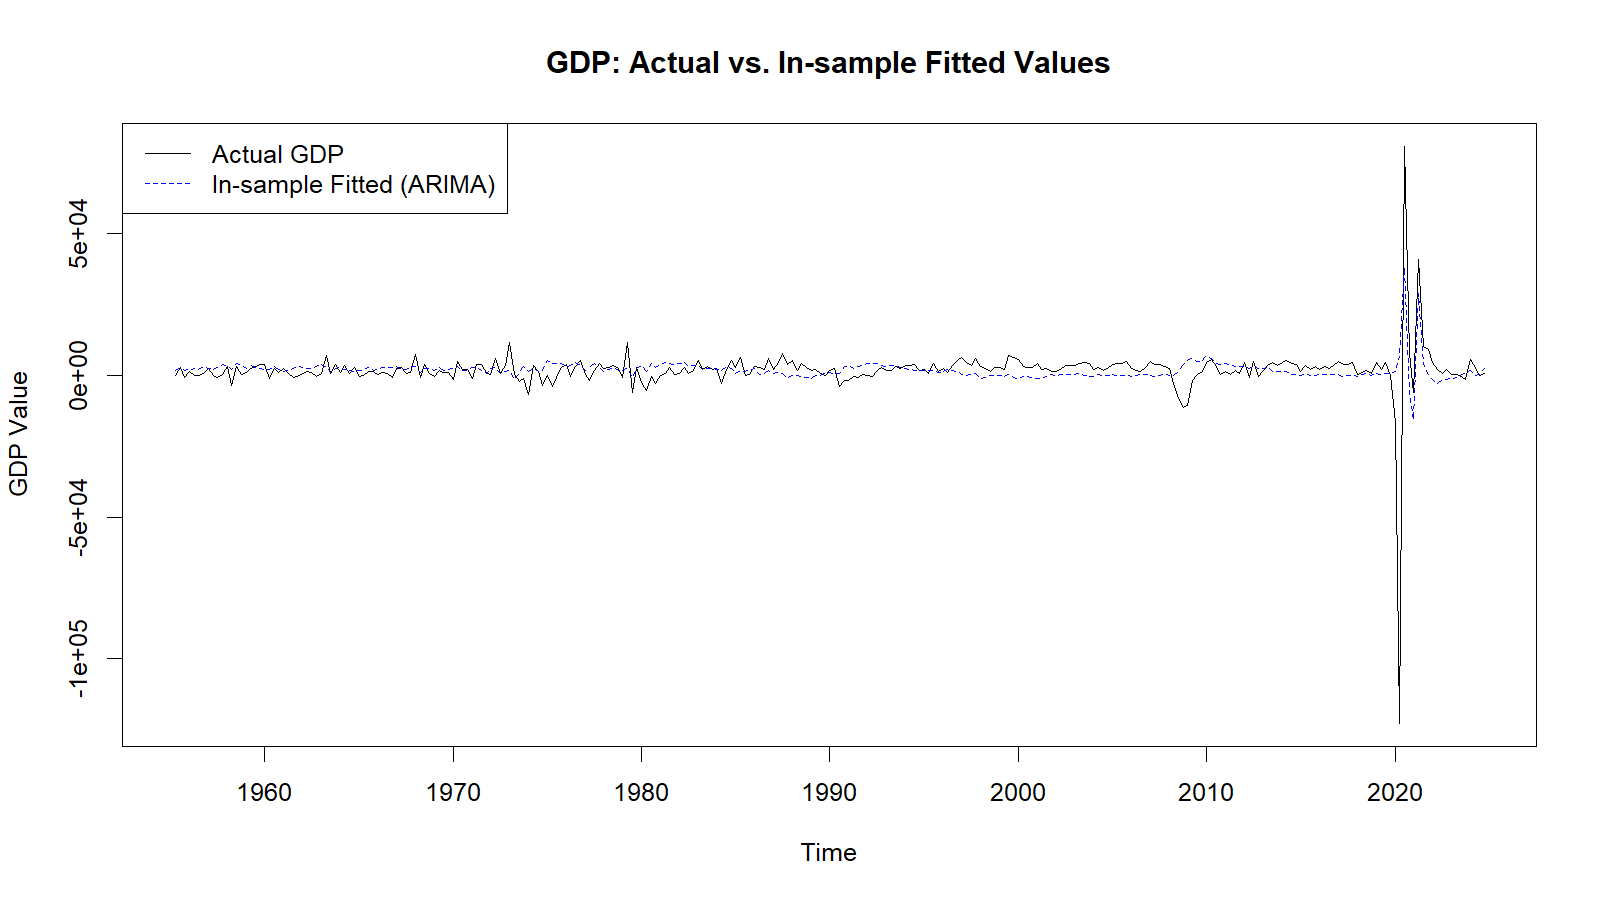
\includegraphics[width=\textwidth]{../figures/GDP_fitted_vs_actual.png}
        \caption{GDP: In-sample forecast}
        \label{fig:gdp_in}
    \end{subfigure}
    \hfill
    \begin{subfigure}[b]{0.45\textwidth}
        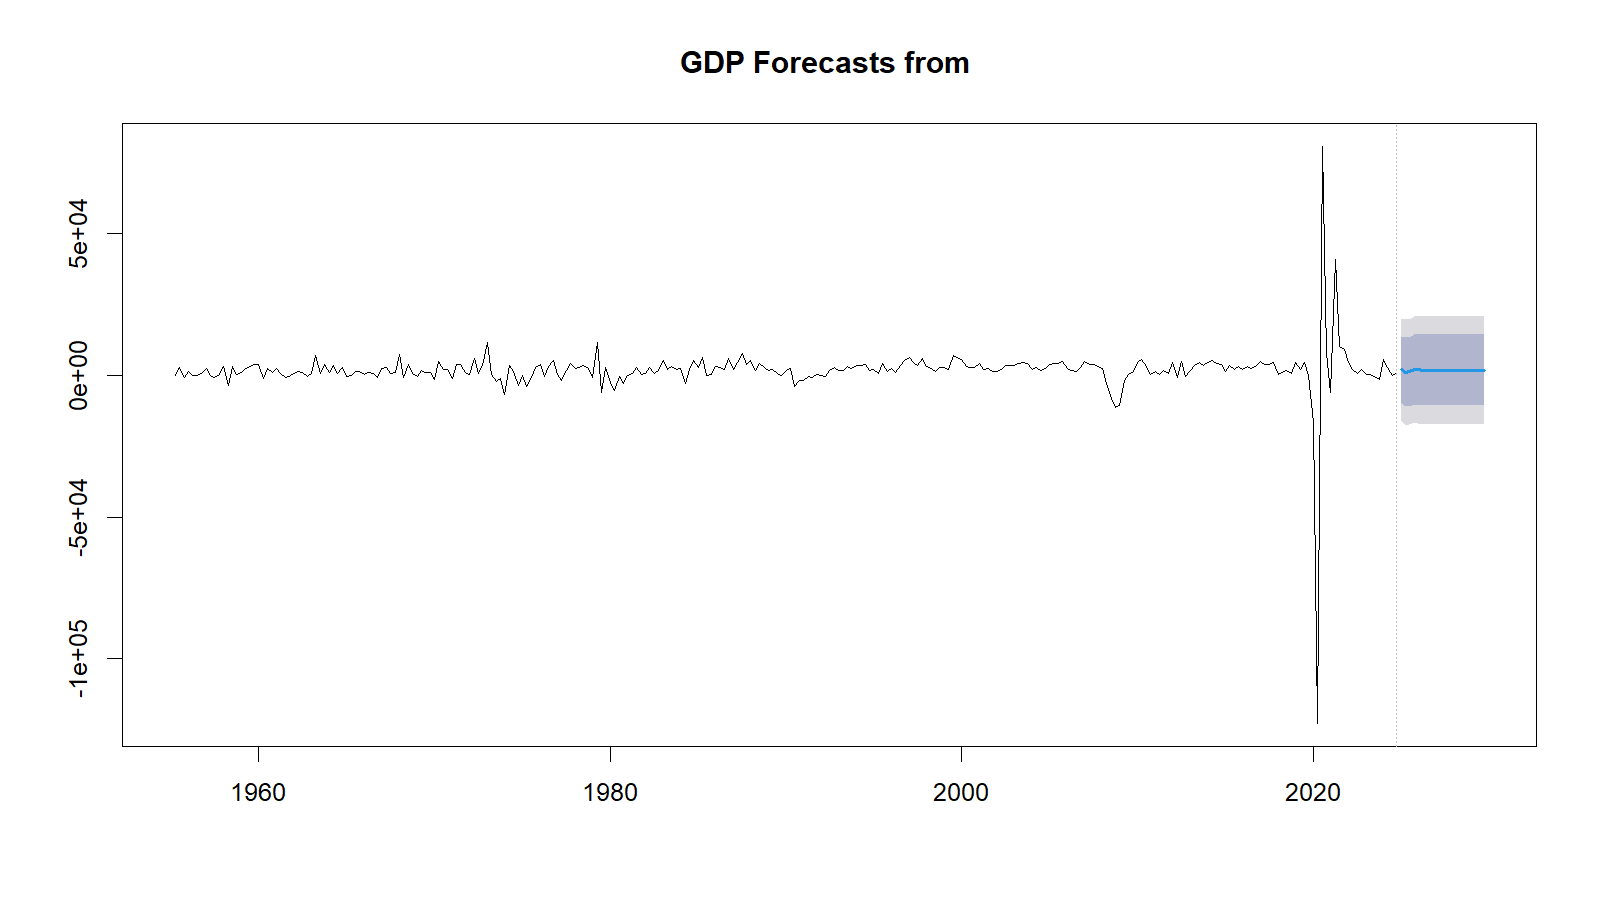
\includegraphics[width=\textwidth]{../figures/GDP_forecast.png}
        \caption{GDP: Out-of-sample forecast}
        \label{fig:gdp_out}
    \end{subfigure}
    
    % Trade Balance: In-sample and Forecast
    \begin{subfigure}[b]{0.45\textwidth}
        \includegraphics[width=\textwidth]{../figures/Trade Balance_fitted_vs_actual.png}
        \caption{Trade Balance: In-sample forecast}
        \label{fig:tb_in}
    \end{subfigure}
    \hfill
    \begin{subfigure}[b]{0.45\textwidth}
        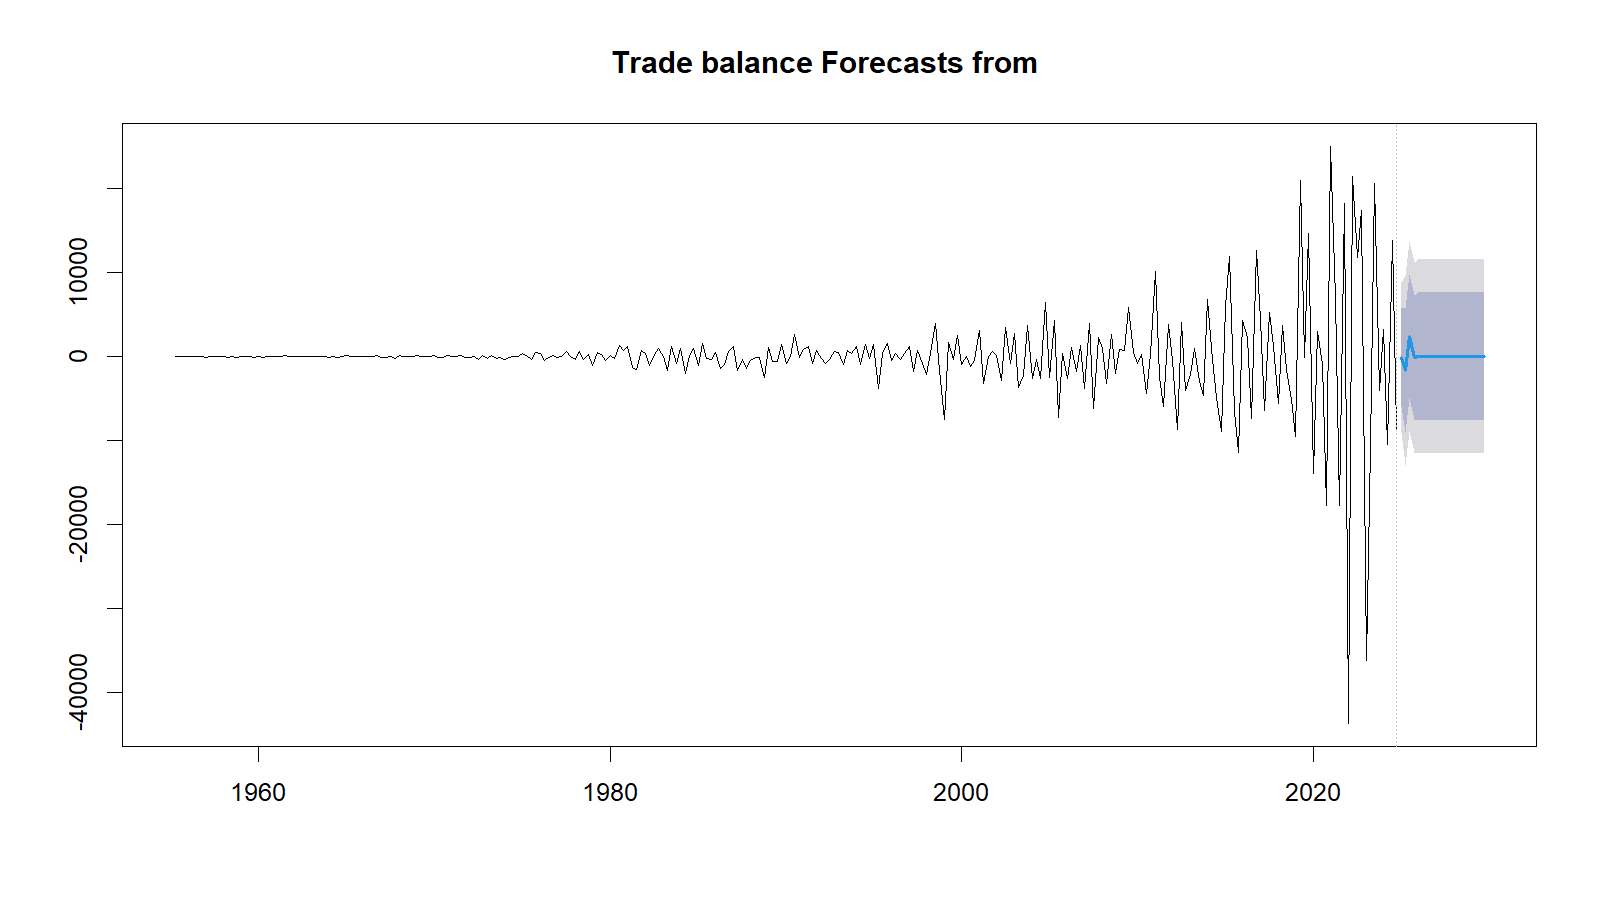
\includegraphics[width=\textwidth]{../figures/Trade Balance_forecast.png}
        \caption{Trade Balance: Out-of-sample forecast}
        \label{fig:tb_out}
    \end{subfigure}
    
    % Exchange Rate: In-sample and Forecast
    \begin{subfigure}[b]{0.45\textwidth}
        \includegraphics[width=\textwidth]{../figures/Exchange Rate_fitted_vs_actual.png}
        \caption{Exchange Rate: In-sample forecast}
        \label{fig:er_in}
    \end{subfigure}
    \hfill
    \begin{subfigure}[b]{0.45\textwidth}
        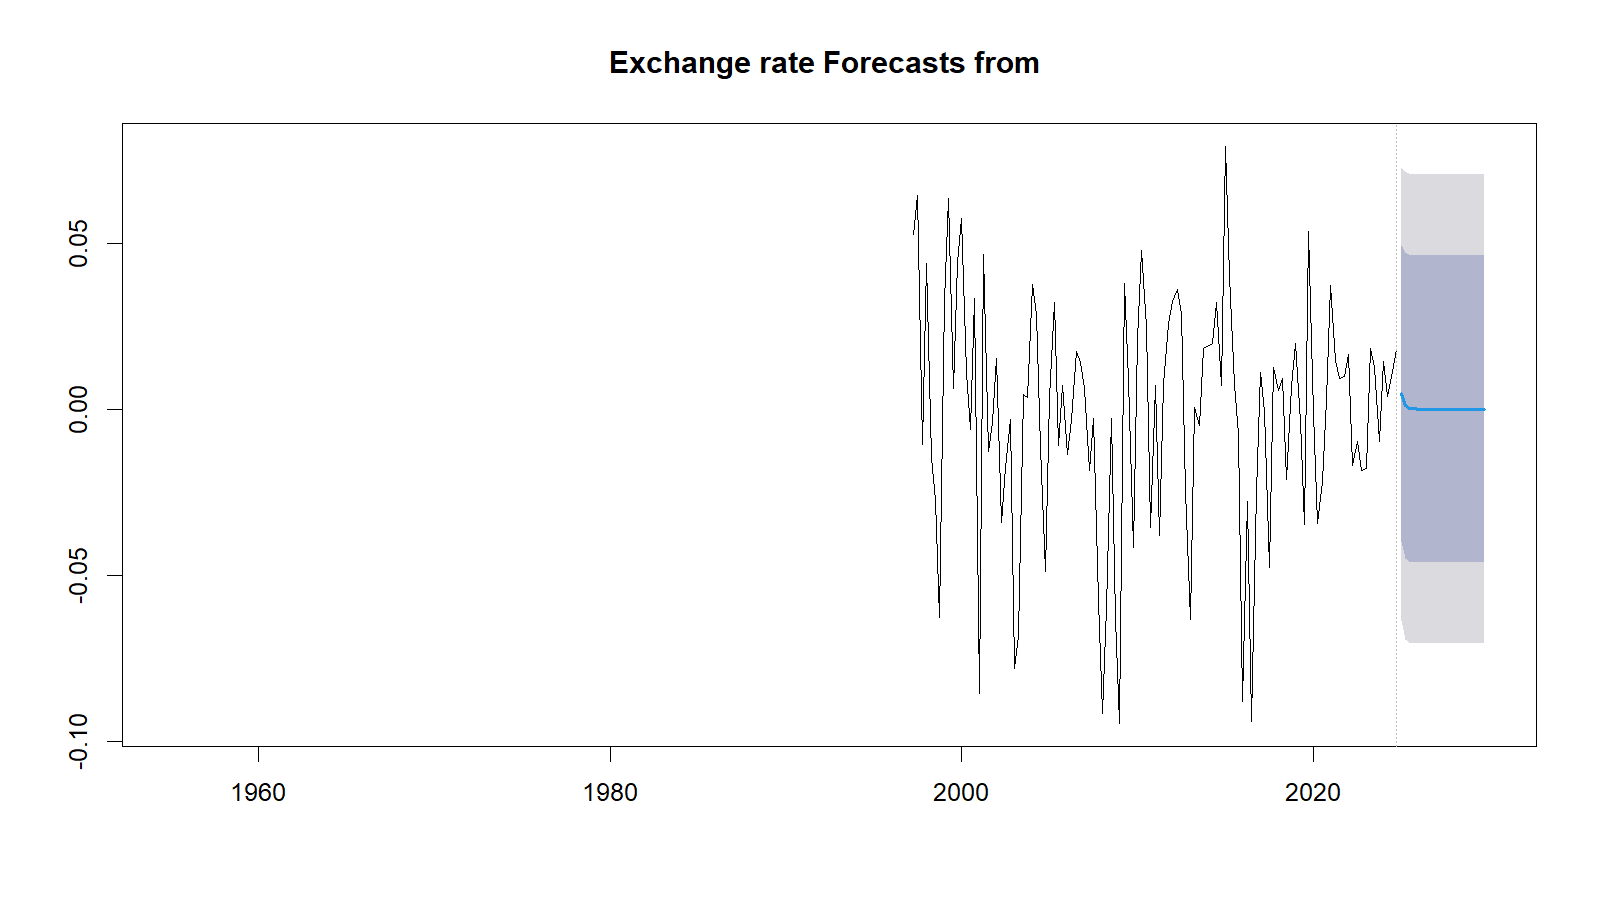
\includegraphics[width=\textwidth]{../figures/Exchange Rate_forecast.png}
        \caption{Exchange Rate: Out-of-sample forecast}
        \label{fig:er_out}
    \end{subfigure}
\end{figure}

\section{Multivariate Analysis}

\subsection{Theoretical framework}

Present a simple model based on paper to guide our analysis especially the 
var ordering for cholesky decomp.

\subsection{Optimal lag selection}

We use the VARselect command in R to estimate the optimal lags. The results in 
table \ref{fig:lagselection} present the optimal lags as suggested by four different tests. These
tests aim to balance out the goodness-of-fit against model complexit with lower 
values indicating better models. While AIC 
(Akaike Information Criterion) and FPE (Final Prediction Error) impose a constant
penalty per additional coefficient (and hence, lag) added to the model, they opt
for more complex dynamics if that means reducing the residual variance. 
By contrast, SC (Schwarz Information Criterion, also known as Bayesian Information Criterion) 
and HQ (Hannan-Quinn) have penalties that increase with the number of lags used, 
hence selecting only the most essential lags. 

\begin{table}[ht]
\centering
\begin{threeparttable}
\caption{\textsc{Optimal Lag Selection Based on Information Criteria}}\label{fig:lagselection}
\begin{tabular}{lc}
 \\[-1.8ex]  \hline \hline  \\[-1.8ex] 
{Criterion} & {Optimal Lag} \\
\midrule
 Akaike Information Criterion (AIC) & 7 \\
Hannan-Quinn Information Criterion (HQ)  & 1 \\
Schwarz Criterion (SC) / Bayesian Information Criterion (BIC)  & 1 \\
Final Prediction Error (FPE) & 7 \\
\hline \hline  \\[-1.8ex] 
\end{tabular}
\end{threeparttable}
\begin{minipage}{\textwidth}
\footnotesize
\textit{Notes:} Coefficient estimates (Coeff.) with standard errors (SE). 
{--} = Component not included in model. Significance levels: $^{***}p<0.01$, $^{**}p<0.05$, $^{*}p<0.1$. 
AR = Autoregressive term, MA = Moving Average term. GDP intercept in original units. 
\textit{Source:} Author's calculations using UK Statistical Office data.
\end{minipage}
\end{table}
This explains why AIC and FPE suggest
7 lags while SC and HQ suggest only 1 lag. In the following, we go with AIC’s and 
FPE’s results using 7 lags for our analysis. Our rationale is its widespread 
use in the econometric modeling literature and its 
robustness in capturing model fit while penalizing complexity less stringently 
than SC or HQ. This makes AIC  particularly suitable for applications 
where predictive accuracy is prioritized, as it allows for a slightly more 
flexible model specification, which is often beneficial in a context 
with potential structural nuances.

\subsection{VAR Estimation}

\paragraph*{Statistical model.}

In R, we estimate the model using the VAR command, which when using 7 lags implies an OLS regression of the following kind: 
\begin{align*}
x_{i,t}=\alpha_{i,0} \sum_{i=1}^3\sum_{k=1}^7\alpha_{i,t-k}x_{i,t-k} + u_{i,t}
\end{align*}
In this equation, $i\in\{1,2,3\}$ stands for GDP, Trade Balance, and Exchange Rate respectively. 

\subsection{Residual testing}

Testing our residuals as shown in Table (??) shows that there is neither serial 
autocorrelation nor conditional heteroscedasticity (ARCH Effects) left in our model. 
However, the normality tests strongly rejects Gaussianity of our error terms suggesting 
that the residual distribution exhibits non-Gaussian features such as heavy tails or 
skewness, implying that standard t-tests and confidence intervals may be invalid 
unless we use sufficiently robust inference methods. This issue is common in VAR models and hence does not alarm us too much.


The test statistics for the behavior of our residuals are summarized in
the following table:

\bgroup \table[H]
\centering
\caption{\label{tab:unnamed-chunk-22}Residuals tests}
\centering
\begin{tabular}[t]{lrrr}
\toprule
Test & ChiSq & df & p.value\\
\midrule
Serial Correlation & 70.6377 & 45 & 0.0086591\\
ARCH & 290.9468 & 288 & 0.4403334\\
Normality & 7261.2574 & 6 & 0.0000000\\
\bottomrule
\end{tabular}
\endtable\egroup

\subsection{VAR forecasts}

Our out-of-sample forecasts for $\Delta$ GDP remain tightly centred on zero—consistent 
with the stationary behavior we established in our VAR—while the fan chart’s 
gradually widening bands reflect the growing uncertainty as the forecast 
horizon extends. Importantly, even after the dramatic COVID-19 shock in early 
2020, the model shows a rapid return of quarterly GDP growth to its long-run 
average of essentially zero, underscoring both the economy’s resilience and 
the appropriateness of our stationary specification.

\begin{figure}

{\centering 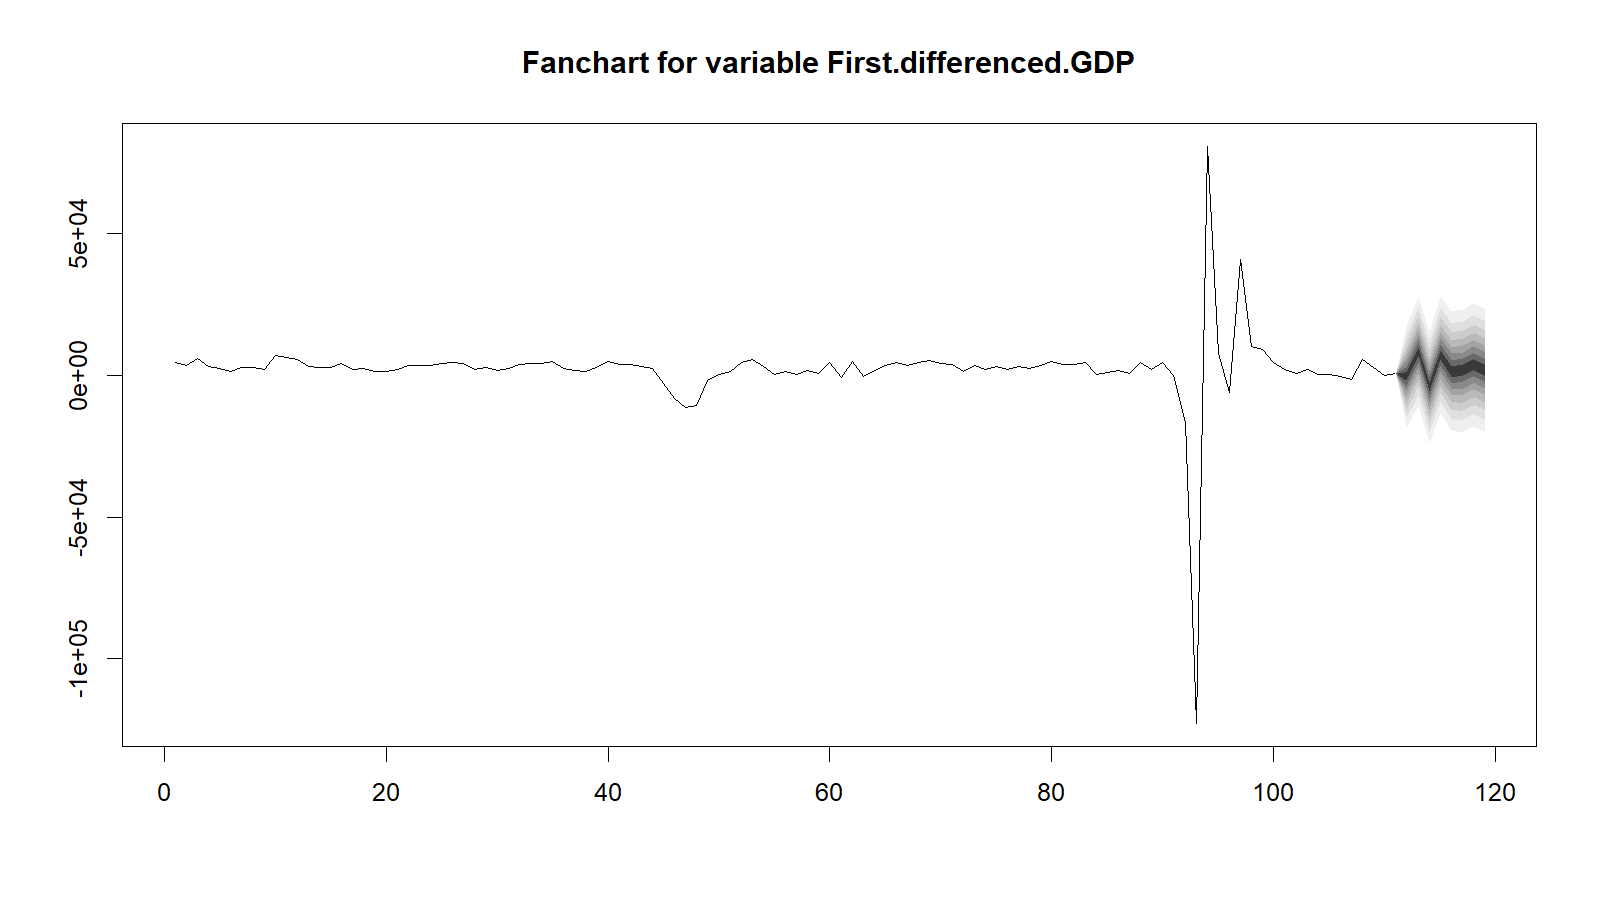
\includegraphics[width=0.8\linewidth]{../figures/VAR_forecast2} 

}

\caption{GDP - VAR Forecast}\label{fig:unnamed-chunk-23}
\end{figure}

\subsection{Cholesky decomposition}

The Cholesky decomposition factorizes the residual covariance matrix of our 
VAR into a lower‐triangular matrix, which yields a set of orthogonal
(i.e. uncorrelated) structural shocks. By imposing a recursive identification
scheme—where the first variable is assumed to be contemporaneously exogenous, 
the second may respond immediately to the first, the third to the first two,
and so on—we obtain a uniquely defined causal ordering. This ordering lets us 
interpret each impulse‐response function as the dynamic effect of a one‐unit 
shock in one variable on all others in the system. In our analysis, we apply 
the Cholesky decomposition to the VAR residuals and adopt the 
ordering: $\Delta$ GDP \textrightarrow Exchange Rate \textrightarrow Trade Balance, 
so that shocks to  $\Delta$ GDP are treated as exogenous and shocks to Trade Balance 
may reflect contemporaneous feedback from both $\Delta$ GDP and Exchange Rate.

\subsection{Impulse response functions}

A natural way to think about the very short‐run causal ordering is that GDP 
shocks—say a surprise shift in domestic demand or productivity—are the 
“slowest moving” of the three: they show up in quarterly national‐accounts 
data and take a full quarter to be measured, and they reflect broad real‐economy
fundamentals. By contrast, the exchange rate is set in continuous, 
high‐frequency financial markets and will react almost instantaneously to 
any news about output or monetary‐policy surprises. Finally, the trade balance 
is connected to contracts, value chains, etc. that make short-term adjustment 
difficult: export and import contracts, shipping lags and invoicing delays mean
that net‐export volumes likely respond with substantial delay to movements
in both output and the exchange rate.

The impulse response functions for GDP are depicted as:

\begin{figure}

{\centering \includegraphics[width=0.8\linewidth]{../figures/IRF_plots/IRF_to_First.differenced.GDP} 

}

\caption{GDP - Shock reactions}\label{fig:unnamed-chunk-24}
\end{figure}

The impulse response functions for Trade Balance are depicted as:

\begin{figure}

{\centering \includegraphics[width=0.8\linewidth]{../figures/IRF_plots/IRF_to_First.differenced.balance.of.payments} 

}

\caption{Trade Balance - Shock reactions}\label{fig:unnamed-chunk-25}
\end{figure}

The impulse response functions for Exchange Rate are depicted as:

\begin{figure}

{\centering \includegraphics[width=0.8\linewidth]{../figures/IRF_plots/IRF_to_First.differenced.exchange.rate} 

}

\caption{Exchange Rate - Shock reactions}\label{fig:unnamed-chunk-26}
\end{figure}

\subsection{Robustness analysis: modify the ordering of the variables}

After modifying the ordering, the IRFs look as follows:

The impulse response functions for GDP are depicted as:

%\begin{figure}

%{\centering \includegraphics[width=0.8\linewidth]{../figures/IRF_plots2/IRF_to_First.differenced.GDP} 

%}

%\caption{GDP - Shock reactions}\label{fig:unnamed-chunk-27}
%\end{figure}

%The impulse response functions for Trade Balance are depicted as:

%\begin{figure}

%{\centering \includegraphics[width=0.8\linewidth]{../figures/IRF_plots2/IRF_to_First.differenced.balance.of.payments} 

%}

%\caption{Trade Balance - Shock reactions}\label{fig:unnamed-chunk-28}
%\end{figure}

%The impulse response functions for Exchange Rate are depicted as:

%\begin{figure}

%{\centering \includegraphics[width=0.8\linewidth]{../figures/IRF_plots2/IRF_to_First.differenced.exchange.rate} 

%}

%\caption{Exchange Rate - Shock reactions}\label{fig:unnamed-chunk-29}
%\end{figure}

\section{Concluding Remarks}

\end{document}
